\newpage
\section{Suddivisione del lavoro} \label{SuddivisioneDelLavoro}
	
	La sezione riporta la ripartizione dei ruoli tra i membri del team di sviluppo, basandosi su quanto pianificato.
	
	Vengono seguite le seguenti regole:
	\begin{itemize}
		\item Ogni membro deve ricoprire ogni ruolo pianificato almeno una volta
		\item Il numero minimo di ore per ruolo che viene ricoperto da un membro in un dato periodo viene fissato a 5 ore
		\item Le ore di lavoro svolte da ogni membro per ogni ruolo dovrà essere più o meno equivalente
     \end{itemize}
     
     Nel preventivo le ore di lavoro impiegate per la \gloss{formazione} personale non vengono rendicontate.
	
	\newpage
	
	\subsection{Dettaglio Fasi}
		\subsubsection{Analisi dei Requisiti}
			La suddivisione dei ruoli tra i vari membri del team di sviluppo nel periodo di Analisi dei Requisiti è la seguente:
			
			\begin{table}[H]
				\begin{detailtable}{\columnwidth}{m{3cm}YYYYYYY}
					\thead{Membro} & 
					\thead{Re} &
					\thead{Am} &
					\thead{An} &
					\thead{Pj} &
					\thead{Pr} &
					\thead{Ve} &
					\thead{Totale}\\\toprule
					\rowcolor{\tablegray}
					\CV & 8 & & 9 & & & 7 & 24 \\
					\LC & & 8 & 9 & & & 7 & 24 \\\rowcolor{\tablegray}
					\MM & 8 & & 9 & & & 7 & 24 \\
					\NC & 8 & & 9 & & & 7 & 24 \\\rowcolor{\tablegray}
					\SG & & 8 & 9 & & & 7 & 24 \\ 
					\TG & & 8 & 9 & & & 7 & 24 \\\bottomrule
				\end{detailtable}
				\caption{Suddivisione oraria nel periodo di Analisi dei Requisiti}
			\end{table}
			
			\begin{figure}[H]
					\centering
					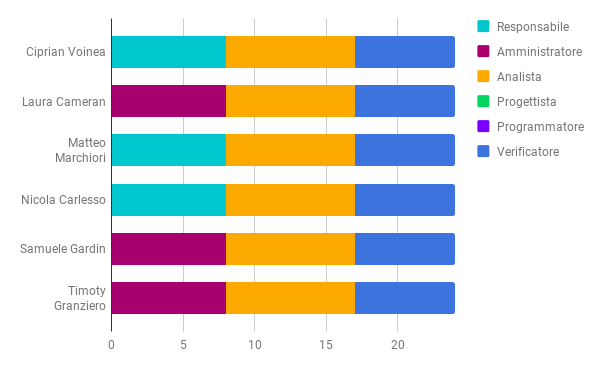
\includegraphics[scale=0.7]{img/Ore_Analisi_dei_Requisiti.png}\\
					\caption{Diagramma di suddivisione del lavoro nel periodo di Analisi dei Requisiti}
			\end{figure}
		
		\newpage
		
		\subsubsection{Progettazione della Base Tecnologica}
			La suddivisione dei ruoli tra i vari membri del team di sviluppo nel periodo di Progettazione della Base Tecnologica è la seguente:
			
			\begin{table}[H]
				\begin{detailtable}{\columnwidth}{m{3cm}YYYYYYY}
					\thead{Membro} & 
					\thead{Re} &
					\thead{Am} &
					\thead{An} &
					\thead{Pj} &
					\thead{Pr} &
					\thead{Ve} &
					\thead{Totale}\\\toprule
					\rowcolor{\tablegray}
					\CV & & 6 & & 20 & & 14 & 40\\
				    \LC & 7 & & 7 & 13 & & 23 & 50\\\rowcolor{\tablegray}
					\MM & & & & 19 & 23 & 7 & 49\\
					\NC & & 7 & & 20 & 10 & 7 & 44\\\rowcolor{\tablegray}
					\SG & 8 & & & 13 & 17 & 7 & 45\\
					\TG & 7 & 7 & 7 & 15 & & 7 & 43\\\bottomrule
				\end{detailtable}
				\caption{Suddivisione oraria nel periodo di Progettazione della Base Tecnologica}
			\end{table}
			
			\begin{figure}[H]
					\centering
					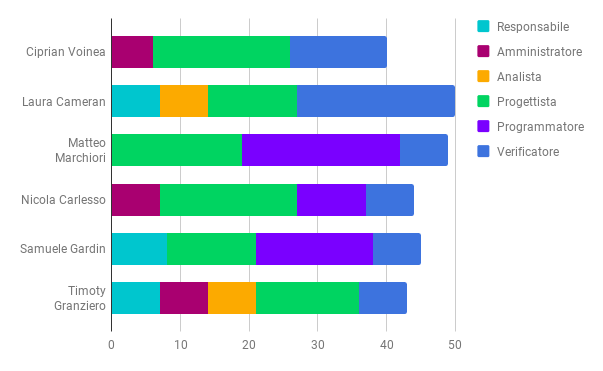
\includegraphics[scale=0.7]{img/Ore_Progettazione_Architetturale.png}\\
					\caption{Diagramma di suddivisione del lavoro nel periodo di Progettazione della Base Tecnologica}
			\end{figure}
			
		\newpage
		
		\subsubsection{Progettazione di Dettaglio e Codifica}
			La suddivisione dei ruoli tra i vari membri del team di sviluppo nel periodo di Progettazione di Dettaglio e Codifica è la seguente:
		
			\begin{table}[H]
				\begin{detailtable}{\columnwidth}{m{3cm}YYYYYYY}
					\thead{Membro} & 
					\thead{Re} &
					\thead{Am} &
					\thead{An} &
					\thead{Pj} &
					\thead{Pr} &
					\thead{Ve} &
					\thead{Totale}\\\toprule
					\rowcolor{\tablegray}
					\CV & & 6 & & 7 & 20 & 10 & 43\\
					\LC & 7 & & & 13 & 21 & & 41\\\rowcolor{\tablegray}
					\MM & 7 & 6 & & 8 & & 21 & 42\\
					\NC & 8 & & & 7 & 11 & 21 & 47\\\rowcolor{\tablegray}
					\SG & & 8 & & 16 & & 21 & 45\\
					\TG & & & & 14 & 17 & 11 & 42\\\bottomrule	
				\end{detailtable}
				\caption{Suddivisione oraria nel periodo di Progettazione di Dettaglio e Codifica}
			\end{table}
			
			\begin{figure}[H]
					\centering
					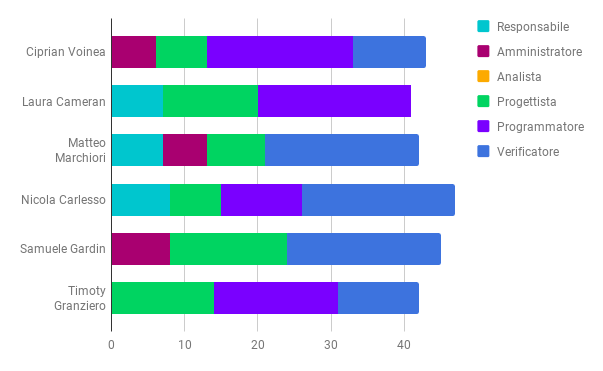
\includegraphics[scale=0.7]{img/Ore_Progettazione_Dettaglio_Codifica.png}\\
					\caption{Diagramma di suddivisione del lavoro nel periodo di Progettazione di Dettaglio e Codifica}
			\end{figure}
			
		\newpage
		
		\subsubsection{Validazione e Collaudo}
			La suddivisione dei ruoli tra i vari membri del team di sviluppo nel periodo di Validazione e Collaudo è la seguente:
			
			\begin{table}[H]
				\begin{detailtable}{\columnwidth}{m{3cm}YYYYYYY}
					\thead{Membro} & 
					\thead{Re} &
					\thead{Am} &
					\thead{An} &
					\thead{Pj} &
					\thead{Pr} &
					\thead{Ve} &
					\thead{Totale}\\\toprule\rowcolor{\tablegray}
					\CV & 8 & & & & & 13 & 21\\
					\LC & & 5 & & & & 8 & 13\\\rowcolor{\tablegray}
					\MM & & 5 & & & & 8 & 13\\
					\NC & & 5 & & & & 8 & 13\\\rowcolor{\tablegray}
					\SG & 6 & & & & & 8 & 14\\
					\TG & 6 & & & & & 13 & 19\\\bottomrule	
				\end{detailtable}
				\caption{Suddivisione oraria nel periodo di Validazione e Collaudo}
			\end{table}
			
			\begin{figure}[H]
					\centering
					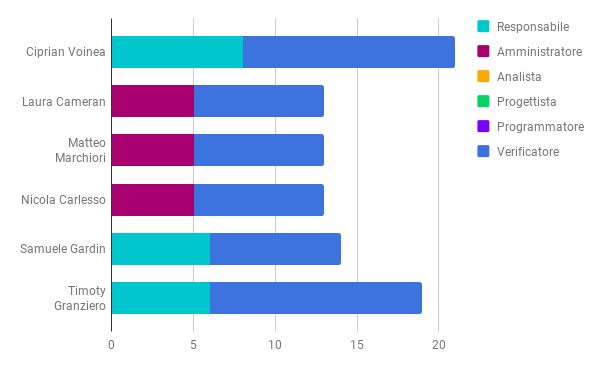
\includegraphics[scale=0.7]{img/Ore_Verifica_Validazione.png}\\
					\caption{Diagramma di suddivisione del lavoro nel periodo di Validazione e Collaudo}
			\end{figure}
			
	\newpage

	\subsection{Totali}
		\subsubsection{Ore totali rendicontate}
			Vengono riportate in seguito i totali delle ore rendicontate in preventivo a carico del \gloss{committente}.
			
			\begin{table}[H]
				\begin{detailtable}{\columnwidth}{m{3cm}YYYYYYY}
					\thead{Membro} & 
					\thead{Re} &
					\thead{Am} &
					\thead{An} &
					\thead{Pj} &
					\thead{Pr} &
					\thead{Ve} &
					\thead{Totale}\\\toprule
					\rowcolor{\tablegray}
					\CV & 8 & 12 & & 27 & 20 & 37 & 104\\
					\LC & 14 & 5 & 7 & 26 & 21 & 31 & 104\\\rowcolor{\tablegray}
					\MM & 7 & 11 & & 27 & 23 & 36 & 104\\
					\NC & 8 & 12 & & 27 & 21 & 36 & 104\\\rowcolor{\tablegray}
					\SG & 14 & 8 & & 29 & 17 & 36 & 104\\
					\TG & 13 & 7 & 7 & 29 & 17 & 31 & 104\\\bottomrule
				\end{detailtable}
				\caption{Ore totali rendicontate}
			\end{table}
			
			\begin{figure}[H]
					\centering
					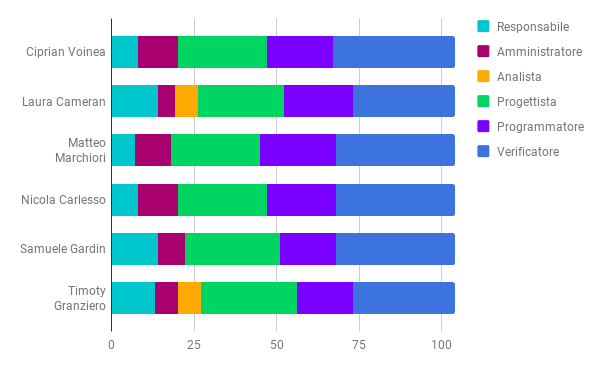
\includegraphics[scale=0.7]{img/Ore_Rendicontate.png}\\
					\caption{Diagramma di confronto con le ore rendicontate}
			\end{figure}
		
		\newpage
	
		\subsubsection{Ore totali con investimento}
			Vengono riportate in seguito i totali delle ore rendicontate in preventivo a carico del committente e delle ore di investimento.
			
			\begin{table}[H]
				\begin{detailtable}{\columnwidth}{m{3cm}YYYYYYY}
					\thead{Membro} & 
					\thead{Re} &
					\thead{Am} &
					\thead{An} &
					\thead{Pj} &
					\thead{Pr} &
					\thead{Ve} &
					\thead{Totale}\\\toprule
					\rowcolor{\tablegray}
					\CV & 20 & 14 & 11 & 31 & 22 & 46 & 144\\
					\LC & 18 & 15 & 11 & 30 & 23 & 40 & 144\\\rowcolor{\tablegray}
					\MM & 19 & 13 & 11 & 31 & 25 & 45 & 144\\
					\NC & 20 & 14 & 11 & 31 & 23 & 45 & 144\\\rowcolor{\tablegray}
					\SG & 18 & 18 & 11 & 33 & 19 & 45 & 144\\
					\TG & 17 & 17 & 18 & 33 & 19 & 40 & 144\\\bottomrule
				\end{detailtable}
				\caption{Ore rendicontate di investimento totali}
			\end{table}
			
			\begin{figure}[H]
					\centering
					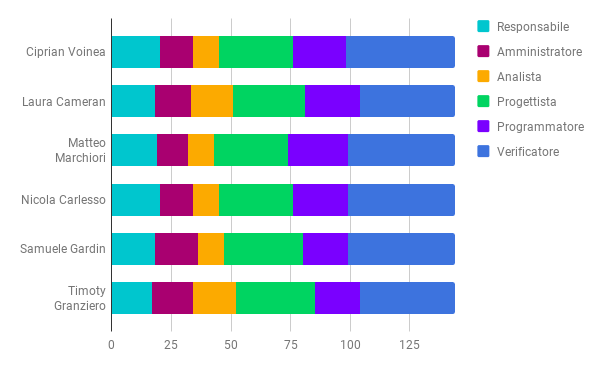
\includegraphics[scale=0.7]{img/Ore_Totali.png}\\
					\caption{Diagramma di confronto con le ore totali}
			\end{figure}
